\newpage
\section{Resultate}
\subsection{Zielerreichung}
Das Projekt OSM Crosswalk Detection barg einige Hürden, von der Schwierigkeit der Bilderkennung, dem Anbinden diverser Schnittstellen und die parallele Verarbeitung grosser Datenmengen.\\
Als Resultat der Arbeit entstand eine Applikation, welche auf Orthofotos Fussgängerstreifen erkennt und deren Koordinaten speichert. Mit Hilfe von OpenStreetMap Daten konnte die Suche auf die Strassenverläufe eingeschränkt werden.
Im Bild unterhalb sind die vom Algorithmus gefundenen Fussgängerstreifen visualisiert. \\
\begin{figure}[H]
\centering
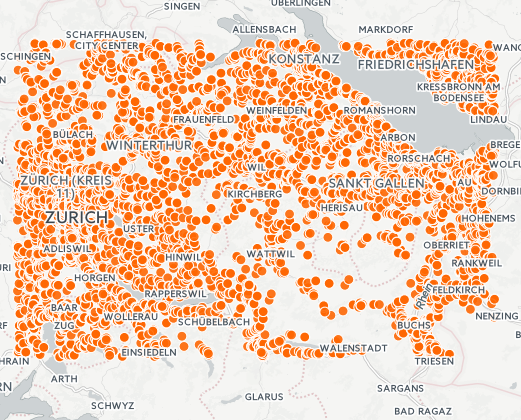
\includegraphics[width=300pt]{images/ostschweiz.png}
\caption[Ostschweiz]{Ostschweiz}
\end{figure}